\newpage
\section{509. 斐波那契数}
\label{leetcode:509}

\subsection{题目}

\textbf{斐波那契数},通常用 F(n) 表示,形成的序列称为\textbf{斐波那契数列}。
该数列由 0 和 1 开始,后面的每一项数字都是前面两项数字的和。也就是:

\begin{verbatim}
  F(0) = 0,   F(1) = 1
  F(N) = F(N - 1) + F(N - 2), 其中 N > 1.
\end{verbatim}

给定 N,计算 F(N)。

\textbf{示例 1}:

\begin{verbatim}
  输入:2
  输出:1
  解释:F(2) = F(1) + F(0) = 1 + 0 = 1.
\end{verbatim}

\textbf{示例 2}:

\begin{verbatim}
  输入:3
  输出:2
  解释:F(3) = F(2) + F(1) = 1 + 1 = 2.
\end{verbatim}

\textbf{示例 3}:

\begin{verbatim}
  输入:4
  输出:3
  解释:F(4) = F(3) + F(2) = 2 + 1 = 3.
\end{verbatim}

\textbf{提示}:

  $0 \leq N \leq 30$

\subsection{题目解析}

这个题目非常重要,后面的爬楼梯,硬币兑换都是这个题目的变种。

DP 方程如下:

  dp[0] = 0 \\
  dp[1] = 1 \\
  dp[i] = dp[i-1] + dp[i-2], $i \geq 2$

\subsection{参考题解,傻递归}

这种方法的状态树巨大,时间复杂度是 O(2$^{n}$)。

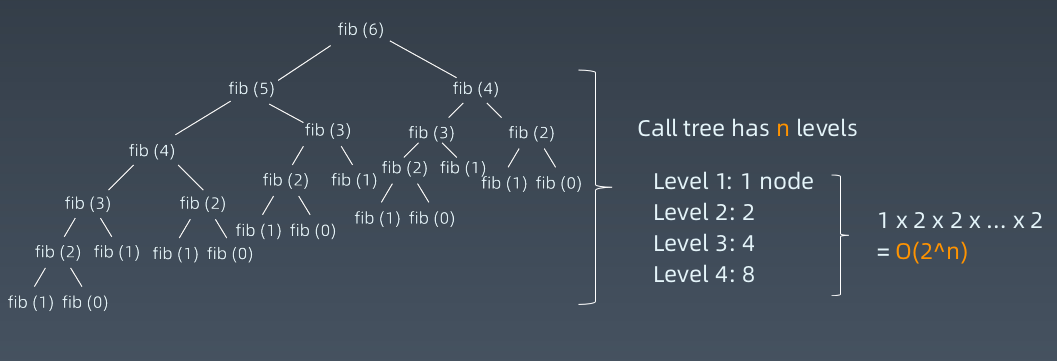
\includegraphics[width=140mm,height=60mm]{images/leetcode/leetcode_509_01.png}

\begin{verbatim}
/**
 * @param {number} N
 * @return {number}
 */
var fib = function(N) {
  if (N < 2) { return N; }
  return fib(N-1) + fib(N-2);
};
\end{verbatim}

\subsection{参考题解,递归+缓存}

时间复杂度为 O(n)。\\
空间复杂度 O(n)。

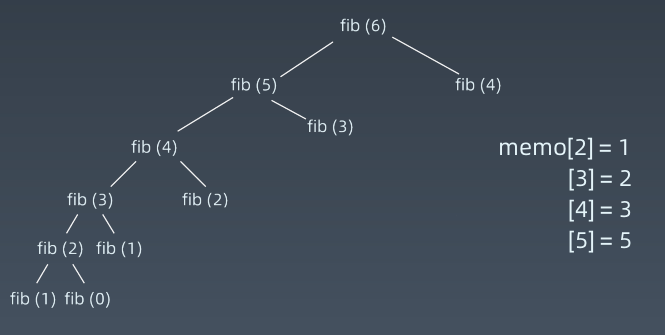
\includegraphics[width=100mm,height=50mm]{images/leetcode/leetcode_509_02.png}

\begin{verbatim}
/**
* @param {number} N
* @return {number}
*/
var fib = function(N) {
  const m = new Map();
  m.set(0, 0);
  m.set(1, 1);
  return recursion(N, m);
};

function recursion(N, m) {
  if (m.has(N)) {
    return m.get(N);
  }
  const result = recursion(N-1, m) + recursion(N-2, m);
  m.set(N, result);
  return result;
}
\end{verbatim}

\subsection{参考题解,递推1}

开辟一个状态数组。

时间复杂度 O(n)。\\
空间复杂度 O(n)。

\begin{verbatim}
/**
* @param {number} N
* @return {number}
*/
var fib = function(N) {
  if (N < 2) { return N; }
  let dp = new Array(N+1);
  dp[0] = 0;
  dp[1] = 1;
  for (let i = 2; i <= N; i += 1) {
    dp[i] = dp[i-1] + dp[i-2];
  }
  return dp[N];
};
\end{verbatim}

\subsection{参考题解,递推经典解法}

上一种解法,你可以看到在 for 循环里面,每次的操作
其实就只涉及到 3 个变量的操作,所以我们其实是可以
不用开辟这个数组的。我们只需要每次循环都保存一下
最新的状态即可。

时间复杂度 O(n)。\\
空间复杂度 O(1)。

\begin{verbatim}
/**
 * @param {number} N
 * @return {number}
 */
var fib = function(N) {
  if (N < 2) {
    return N;
  }
  let f1 = 0;
  let f2 = 1;
  for (let i = 2; i <= N; i += 1) {
    [f1, f2] = [f2, f1 + f2];
  }
  return f2;
};
\end{verbatim}

\subsection{参考题解,查表法}

时间复杂度 O(1)。\\
空间复杂度 O(n)。

\subsection{参考题解,矩阵法}

时间复杂度 O(${\log}_2 n$)。\\
空间复杂度 O(1)。

\subsection{参考题解,通项公式}

时间复杂度 O(1)。\\
空间复杂度 O(1)。
